\subsection{Unsupervised Activity Representation}
\label{basics}
In this section, we explain the generative model which we use in order to jointly learn the activities from videos. We start with explaining the notation. As we already defined in the previous sections, we note the extracted frame representation of the frame $t$ of video $i$ as $\mathbf{y^{(i)}_t}$. Moreover, we model our algorithm based on activities and the note the activity of the $t^{th}$ frame of the $i^{th}$ video as $z^{(i)}_t$. Since our model is non-parametric, the number of activities are not fixed \ie  $z^{(i)}_t \in \mathcal{N}$.


We model each activity as a Bernoulli distribution over the visual and language atoms as $\theta_k=[\theta_k^l,\theta_k^v]$ such that $m^{th}$ entry of the $\theta_k^l$ represents the likelihood of seeing $m^{th}$ language word in the frame having activity $k$. Similarly, $m^{th}$ entry of the $\theta_k^v$ represents the likelihood of seeing $m^{th}$ object. In other words, each frame's representation $\mathbf{y^{(i)}_t}$ is sampled from its activity distribution as \mbox{$\mathbf{y^{(i)}_t}|z^{(i)}_t=k \sim Ber(\theta_k)$}. As a prior over $\theta$, we use its conjugate distribution -- \emph{Beta distribution} --.

In the following sections, we first explain the generative model which links activities and frames. Then, we explain how this model can be jointly learned and inferred by using the combination of Gibbs sampling and Metropolis-Hasting samplers.
\subsubsection{Beta Process Hidden Markov Model}
For joint understanding of the time-series information, Fox et al.\cite{foxBPHMM} proposed the Beta Process Hidden Markov Models (BP-HMM). It relies on the set of features(activities in our case) which can explain the behaviour of all time-series data (all videos in our case). In BP-HMM setting, each time-series data exhibits a subset of available features.

In our model, each video $i$ chooses a set of activities through an activity vector $\mathbf{f^{(i)}}$ such that $f^{(i)}_k$ is $1$ if $i^th$ video has activity $k$, it is 0 otherwise. When the activity vectors of all videos are concatenated, it becomes an activity matrix $\mathbf{F}$ such that $i^th$ row of the $\mathbf{F}$ is the activity vector $\mathbf{f^{(i)}}$. Moreover, each feature $k$ also has a prior probability $b_k$  and a distribution parameter $\theta_k$. Distribution parameter $\theta_k$ is the Bernoulli distribution as explained in the Section \ref{basics}. Moreover, its base distribution ($B_0$) is the \emph{Beta random variable}. In this setting, the activity parameters $\theta_k$ and $b_k$ follow the \emph{beta process} as;
\begin{equation}
  B|B_0,\gamma,\beta \sim \text{BP}(\beta,\gamma B_o), B=\sum_{k=1}^\infty b_k \delta_{\theta_k}
\end{equation}
where $B_0$ and the $b_k$ are determined by the underlying Poisson process \cite{ibp} and the feature vector is determined as independent Bernoulli draws as $f_{k}^{(i)} \sim Ber(b_k)$. After marginalizing over the $b_k$ and $\theta_k$, this distribution is shown to be equivalent to Indian Buffet Process \cite{ibp}. Where videos are customers and activities are dishes in the buffet. The first video chooses a $\text{Poisson}(\gamma)$ unique dishes. The following video $i$ chooses previously sampled activity $k$ with probability $\frac{m_k}{i}$,  proportional to the number of videos ($m_k$) chosen the activity $k$, and it also chooses $\text{Poisson}(\frac{\gamma}{i})$ new activities. Here, $\gamma$ controls the number of selected activities in each video and $\beta$ controls the likelihood of the features getting shared by multiple videos.

After each video chooses a subset of activities, we model the videos as an Hidden Markov Model (HMM) over the selected activities. Each frame has the hidden state activity id($z^{(i)}_t$) and we observe the binary representation $\mathbf{y^{(i)}_t}$. Since we model each activity as a Bernoulli distribution, the emission probabilities follow the Bernoulli distribution as $p(\mathbf{y^{(i)}_t}|z^{(i)}_t)=Ber(\theta_{z^{(i)}_t})$. Following the construction of the Fox et al.\cite{foxBPHMM}, we sample the transition probabilities from a normalized Gamma distribution. For each video $i$, we sample a Gamma random variable for the transition between activity $j$ and activity $k$ if both of the activities are included by the video \ie if $f^i_k$ and $f^i_j$ are both $1$. After sampling these random variables, we normalize them to have proper transition probabilities. This procedure can be represented formally as
\begin{equation}
  \eta_{j,k}^{(i)} \sim Gam(\alpha+\kappa \delta_{j,k},1), \quad \mathbf{\pi_j^{(i)}} = \frac{\mathbf{\eta^{(i)}_j} \circ \mathbf{f^{(i)}}}{\sum_k \eta^{(i)}_{j,k} f^{(i)}_k}
\end{equation}
Where $\kappa$ is the persistence parameter promoting the self state transitions to have more coherent temporal boundaries, $\circ$ is the element-wise product and $\pi^i_j$ is the transition probabilities in video $i$ from state $j$ to all states in the form of a vector. This model is also presented as a graphical model in Figure \ref{bphmmo}
\begin{figure}[h!]
  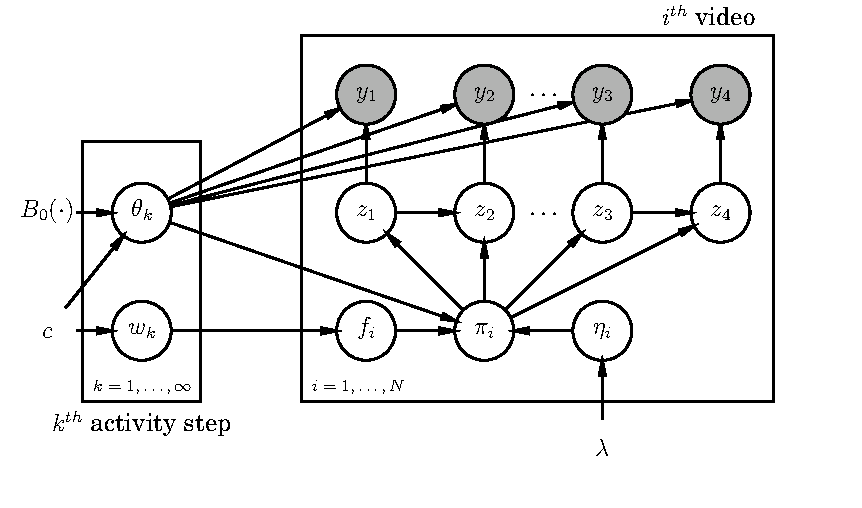
\includegraphics[width=0.5\textwidth]{plate}
  \caption{\textbf{Graphical model for BP-HMM:} The left plate represent the set of activities and right plate represent the set of videos. Each video choose a subset of activities through $\mathbf{f^{(i)}}$ and transition probabilities between them. After the features are selected, the marginal model of the each video becomes an Hidden Markov Model. \emph{See the text for the details.}}
  \label{bphmmo}
\end{figure}


\subsubsection{Gibbs sampling for BP-HMM}
We employ Markov Chain Monte Carlo (MCMC) method for learning and inference of the BP-HMM. We base our algorithms on the MCMC procedure proposed by Fox et al.\cite{foxBPHMM}. Our sampling procedure composed of iterative sampling of activity assignments ($\mathbf{f^{(i)}}$) from the current activity means $\mathbf{\theta_k}$, state assignments $z^{(i)}_t$ and observations $y^{(i)}_k$, and HMM parameters $\mathbf{\eta}$,$\mathbf{\pi}$,$\mathbf{\theta_k}$ from the selected activities $\mathbf{f^{(i)}}$. We give the details of the sampler in the supplementary material.